\scanpage{28}

\mspage{13}

\[
\begin{aligned}
\underset{\substack{\shortparallel\\\mathrm{SL}(2,\mathbb{Z})/{\pm1}}}{\mathrm{SL}(2,\mathbb{Z})'}&\xleftarrow{\overset{\varphi}{\sim}}\mathbb{G}^{\unsure{o|0|\circ}}_{3,\infty}\\
&\quad\deleted{\longleftarrow\rho_0}
\end{aligned}\tag*{(68)}
\]

donné par

\[
\varphi\left\{\begin{aligned}
\rho_1&\longmapsto\inserted{\lambda_1=}\begin{pmatrix}0&1\\-1&0\end{pmatrix}=\sigma^{\deleted{\unsure{\prime}}}\\
\rho_\infty&\longmapsto\inserted{\lambda_\infty=}\begin{pmatrix}1&-1\\1&0\end{pmatrix}=\rho^{\deleted{\unsure{\prime}}-1}\\
\rho_0&\longmapsto\inserted{\lambda_0=}\begin{pmatrix}1&-1\\0&1\end{pmatrix}=\varepsilon_0
\end{aligned}\right\}\ \substack{\deleted{\bmod{\pm1}}\\\bmod{\pm1}}\tag*{(69)}
\]

(suivant un formulaire), qui s'insère d'ailleurs dans un isomorphisme entre

\[
G_{3,\infty}=\{\tau_0,\tau_1,\tau_\infty\mid\tau_0^2=\tau_1^{\unsure{2}}=\tau_\infty^2=(\tau_0\tau_\infty)^2=(\tau_0\tau_1)^3=1\}\tag*{(70)}
\]

% slanted
\margin{\uline{NB}\quad$\begin{aligned}\rho_\infty&=\tau_1\tau_0\\\rho_0&=\tau_\infty\tau_1\\\rho_1&=\tau_0\tau_\infty\end{aligned}$}

et $\mathrm{GL}(2,\mathbb{Z})'=\mathrm{GL}(2,\mathbb{Z})/\{\pm1\}$, savoir

\[
\underset{\substack{\shortparallel\\\mathrm{GL}(\unsure{n|2},\mathbb{Z})/\{\pm1\}}}{\mathrm{GL}(2,\mathbb{Z})'}\xleftarrow{\sim}G_{3,\infty}\tag*{(71)}
\]

\figure{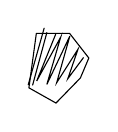
\begin{tikzpicture}[scale=.43,line cap=round]
\draw (.12,2.1)--(1.10,2.10)--(1.67,1.37)--(1.42,.78)--(.70,.04)--(-.10,.49)--(.12,2.1);
\draw (.35,2.25)--(-.12,.58) (.43,2.12)--(.01,.57) (.69,2.07)--(.13,.69)--(.84,1.99)--(.43,.59)--(1.11,2.02)--(.72,.64)--(1.35,1.63)--(1.05,.76)--(1.51,1.38);
\end{tikzpicture}}

donné par

\[
\left\{\begin{aligned}
\tau_{\infty}&\longmapsto\inserted{r_\infty=}\begin{pmatrix}-1&0\\0&1\end{pmatrix}=\tau_\infty\\
\tau_0&\longmapsto\inserted{r_0=}\begin{pmatrix}0&1\\1&0\end{pmatrix}=\tau'_\infty\\
\tau_1&\longmapsto\inserted{r_1=}\begin{pmatrix}-1&\deleted{\unsure{-}}1\\0&1\end{pmatrix}=-\tau'_0
\end{aligned}\right.\tag*{(72)}
\]

\figure{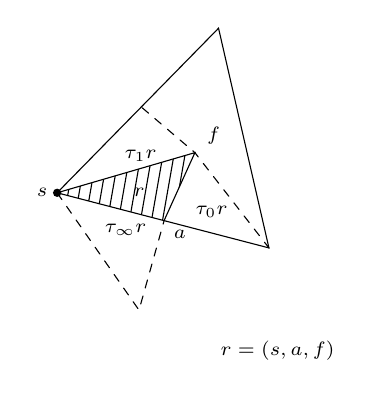
\begin{tikzpicture}[scale=1.0,line cap=round,font=\scriptsize]
\coordinate (s) at (0,.70);\coordinate (v) at (2.05,2.79);\coordinate (w) at (2.69,0);\coordinate (f) at (1.75,1.21);\coordinate (a) at (1.36,.35);\coordinate (q) at (1.04,-.79);
\draw (s)--(v)--(w)--cycle;\draw (s)--(f)--(a);
\begin{scope}\clip (s)--(f)--(a)--cycle;\foreach \x in {0,.14,...,1.75}{\draw (\x,-.1)--++(.28,1.6);}\end{scope}
\draw[dashed] (1.08,1.78)--(f)--(w) (s)--(q)--(a);
\fill (s) circle (1.5pt);\node[left] at (s) {$s$};\node[right] at (1.78,1.43) {$f$};\node[below right] at (a) {$a$};
\node at (1.04,.71) {$r$};\node at (1.06,1.17) {$\tau_1r$};\node at (1.96,.46) {$\tau_0r$};\node at (.87,.23) {$\tau_\infty r$};
\node at (2.80,-1.31) {$r=(s,a,f)$};
\end{tikzpicture}}

\margin{Cf ``formulaire pour $\unsure{\pi_{03}|\mathrm{T}_{03}|\mathrm{Th}_{03}}$ etc''}

% archive sheet number: 27
